\section{RTC}
\label{chap:RTC}
Um die gewonnenen Messdaten mit einem Zeitstempel zu versehen, wird eine \textbf{RTC} (\textit{real time clock}) benötigt. Um eine möglichst kleine Abweichung zu haben, wird eine hohe Präzision vorausgesetzt. Ausserdem soll die \textbf{RTC} über das in Kapitel \ref{subsubsec:I2C} erwähnte \textbf{I$^2$C}-Bus angesteuert werden. Aus diesen Gründen wurde der \textbf{DS3231} implementiert, da dieser als Präzisions-\textbf{I$^2$C}-\textbf{RTC} die Anforderungen erfüllt. Zu sehen ist der \textbf{DS3231} mit seinen Anschlüssen in Abbildung \ref{fig:DS3231}.

\begin{figure}[h]
\centering
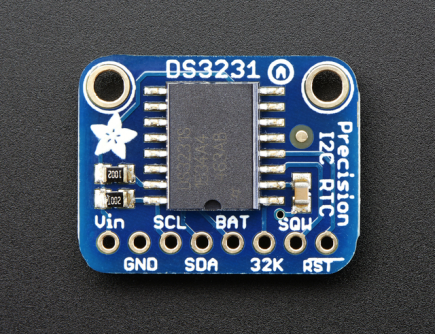
\includegraphics[width=0.6\linewidth]{graphics/DS3231.png}
\caption{DS3231 mit seinen Anschlüssen \cite{Ada2018}.}
\label{fig:DS3231}
\end{figure}